
%%%%%%%%%%%%%%%%%%%%%%%%%%%%%%%%%%%%%%%%%%%%%%%%%%%%%%%%%%%%%%%%%%% 
%                                                                 %
%                           FUTUREWORK                            %
%                                                                 %
%%%%%%%%%%%%%%%%%%%%%%%%%%%%%%%%%%%%%%%%%%%%%%%%%%%%%%%%%%%%%%%%%%% 
 
% \specialhead{FUTUREWORK}
\chapter{FUTURE WORK AND CONCLUSION}
\label{chapter:future_work}

The previous chapter presented the resulting visualization from applying the magnification functions to the graph network and satellite images. The overall performance of the application was also measured to ascertain the viability of using this visualization for larger datasets. This chapter will present a few areas of possible improvement for the current implementation with regards to visual results and algorithm performance.

\section{Satellite Images}
\label{section:future_satellite_images}

The current method of performing linear magnification on the satellite images does not provide the same level of detail of the resulting image as an equivalent global zoom does. This is due to the magnification spreading a relatively small number of texture coordinates over a large area of screen space. Ideally, we would use a method similar to mipmapping where we load the higher resolution textures into GPU memory and use that to provide a greater amount of detail for the magnified
areas. This method was proposed by Keahey as Seamless Multi-Level Views \cite{Keahey1998}.

\begin{figure} \centering
    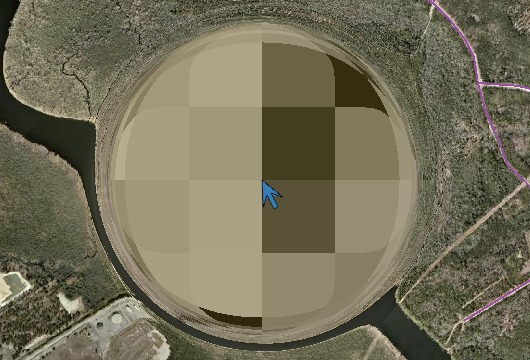
\includegraphics[width=0.50\linewidth]{img/artifacts_clipped.jpg}
    \caption[Satellite Image Magnification Artifacts]{Individual pixels are currently seen with a 72x linear zoom.}
    \label{fig:artifacts_clipped}
\end{figure}

There are a few problems with directly implementing such a technique. There is a limited amount of data that can be stored at any particular resolution on the GPU\@. The amount of memory stored on a GPU averages at about 2 GB\@. As stated previously, the FBO texture takes up approximately 4.5 MB with the application running at a 1600 by 1000 resolution. The FBO is currently used to store any data that is not immediately rendered as textures. 2D textures are limited within OpenGL by their
larger dimension, this value ranges from 1024 to 16384, depending on the hardware. If we have twice the level of detail of a region, we must take up four times as much data in the resulting texture if we wish to store the same geographic coordinates as the lower level of detail image. This magnified region could be generated as the cursors move around the application, but that requires the operations to be fast enough
to calculate every possible discrete level of detail that the cursors can use. The current cursors move to fast with respect to geographic positions, so once this has been addressed, the system would not need to update these extra regions as often. We could also use the lower resolution texture as an option until the higher resolution one has been made available.

While seeing the individual pixels helps the user understand how much they are magnifying the source texture, it obscures any finer details about the geography that might be useful information. Being able to see more detail is the priority of performing magnification. Other effects can be added to help indicate the intensity of a magnification, as suggested by Keahey \cite{Keahey1998}.

The road networks, similar to the satellite images, are also heavily pixelated in the resulting magnification. This can be fixed by simply rendering the road network to the screen instead of to the FBO. 

\begin{figure} \centering
    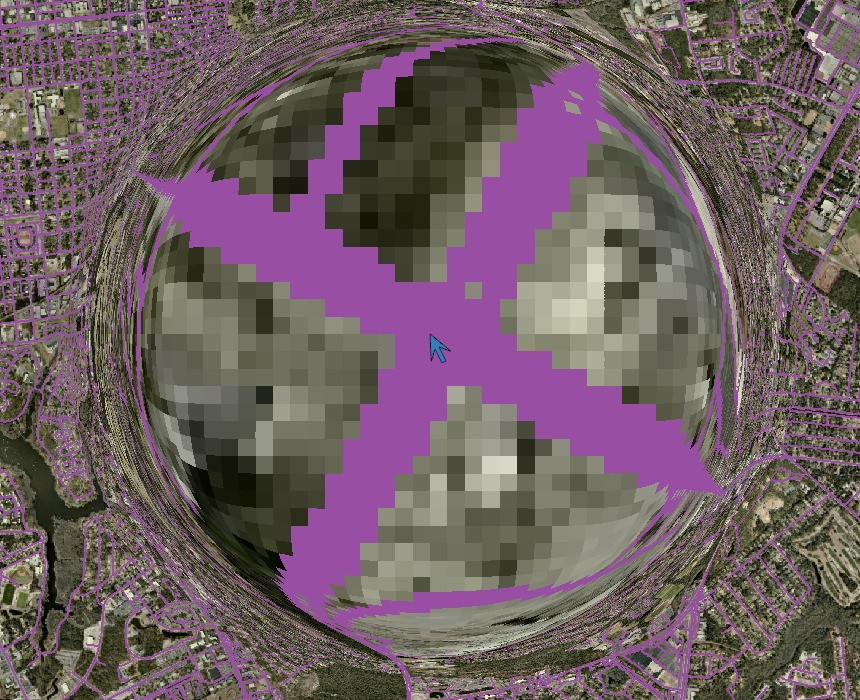
\includegraphics[width=0.50\linewidth]{img/aliasing_clip.jpg}
    \caption[Road Network Artifacts]{The aliasing of the road network is seen due to the 17.4x linear zoom.}
    \label{fig:aliasing_clipped}
\end{figure}

Combined magnification regions caused by overlapping mouse cursors for satellite images produce some odd results. An example is seen in Figure~\ref{fig:distortion_clipped}. It is unclear what should happen when two regions are combined for our applications, it may be correct to prevent different cursors from interacting with each other to avoid creating any sort of extreme satellite distortion. A few options for combining areas of magnification were presented by Keahey and Robertson, including weighted
averages and maximal ray clipping \cite{Keahey1996}.

\begin{figure} \centering
    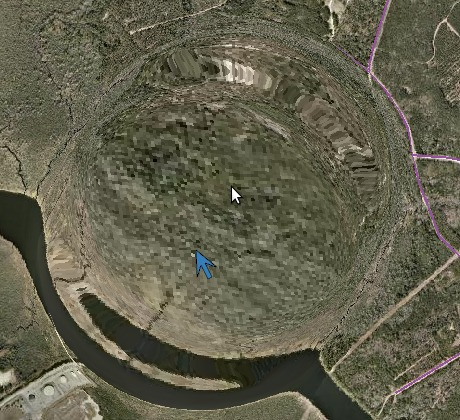
\includegraphics[width=0.50\linewidth]{img/added_distortion_clip.jpg}
    \caption[Combined Satellite Distortion]{An image showing two combined areas of 6.7x magnification. The continuous river south of the cursors does not contain a branch in the original image.}
    \label{fig:distortion_clipped}
\end{figure}

\section{Graph Network}
\label{section:future_graph_network}

Combined areas of magnification do not currently result in graph elements being placed in the same geographic location due to an algorithmic error. This is due to a difference in the premise behind the texture magnification and the graph magnification. The algorithm for texture magnification calculates what geographic data should go at a particular screen location, while the graph magnification tells graph elements to move to a screen location. To move the elements of the graph correctly, we must apply the movement operation to the graph multiple times for each cursor until the same result is obtained twice. 

We can avoid the incorrect placement of graph elements by changing the interaction between areas of magnification. When areas of magnification overlap, we can have the application respond by having the cursors stay in the same screen position but display different geographic and graph information. Another possibility is performing magnification on the convex shape or line formed by elements whose areas of magnification overlap.

As mentioned previously in Chapter~\ref{chapter:results}, the graph movement operations are inefficient for large amounts of data. The current set of graph operations rely on a quad tree implementation which could be used to avoid measuring the distance to every element within the graph. While this quad tree implementation would not improve performance where a large amount of nodes are in a single area, the fact that the data is geographic ensures that this situation is rare.

\section{Conclusion}
\label{section:conclusion}

Creating a focus plus context visualization of data is highly dependent on what information needs to be displayed. For the Infrastructure Visualization, we opt to use a region of non-linear magnification surrounding a region of linear magnification to keep as much context of the data as possible. This thesis explained the necessary changes to the existing visualization to transition to modern OpenGL to perform these functions on our data. We presented techniques for applying
this magnification to both the satellite data and the geographically-based graph data to ensure that the data remained consistent visually. These functions are currently
efficient enough to support a system with 20,000 elements and run in real time.
